%%%%%%%%%%%%%%%%%%%%%%%%%%%%%%%%%
\subsection{Introduction}
\label{sec:fddp-slow-cryo-intro}


% identical between SP and DP 
The Cryogenic Instrumentation and Slow Controls (CISC) system provides a comprehensive monitoring and control system for all detector components and cryogenic instrumentation for the cryostat interior. The subsystems included within the cryogenic instrumentation system are purity monitors, temperature monitors, gas analyzers, liquid argon level monitors, cameras, cryogenic instrumentation test facility and cryogenic piping inside the cryostat. The slow controls system includes four main components: hardware, infrastructure, software and firmware. The slow controls hardware and infrastructure consists of networking hardware, signal processing hardware, computing hardware and relevant rack infrastructure. The slow controls software and firmware will be needed for signal processing, alarms, archiving and control room displays. A subsystem chart for the CISC system is shown in Fig.\ \ref{fig:dp-slow-cryo-subsys}.

\begin{dunefigure}[Cryogenic Instrumentation and Slow Controls (CISC) subsystems]{fig:dp-slow-cryo-subsys}
{Cryogenic Instrumentation and Slow Controls (CISC) subsystem chart}
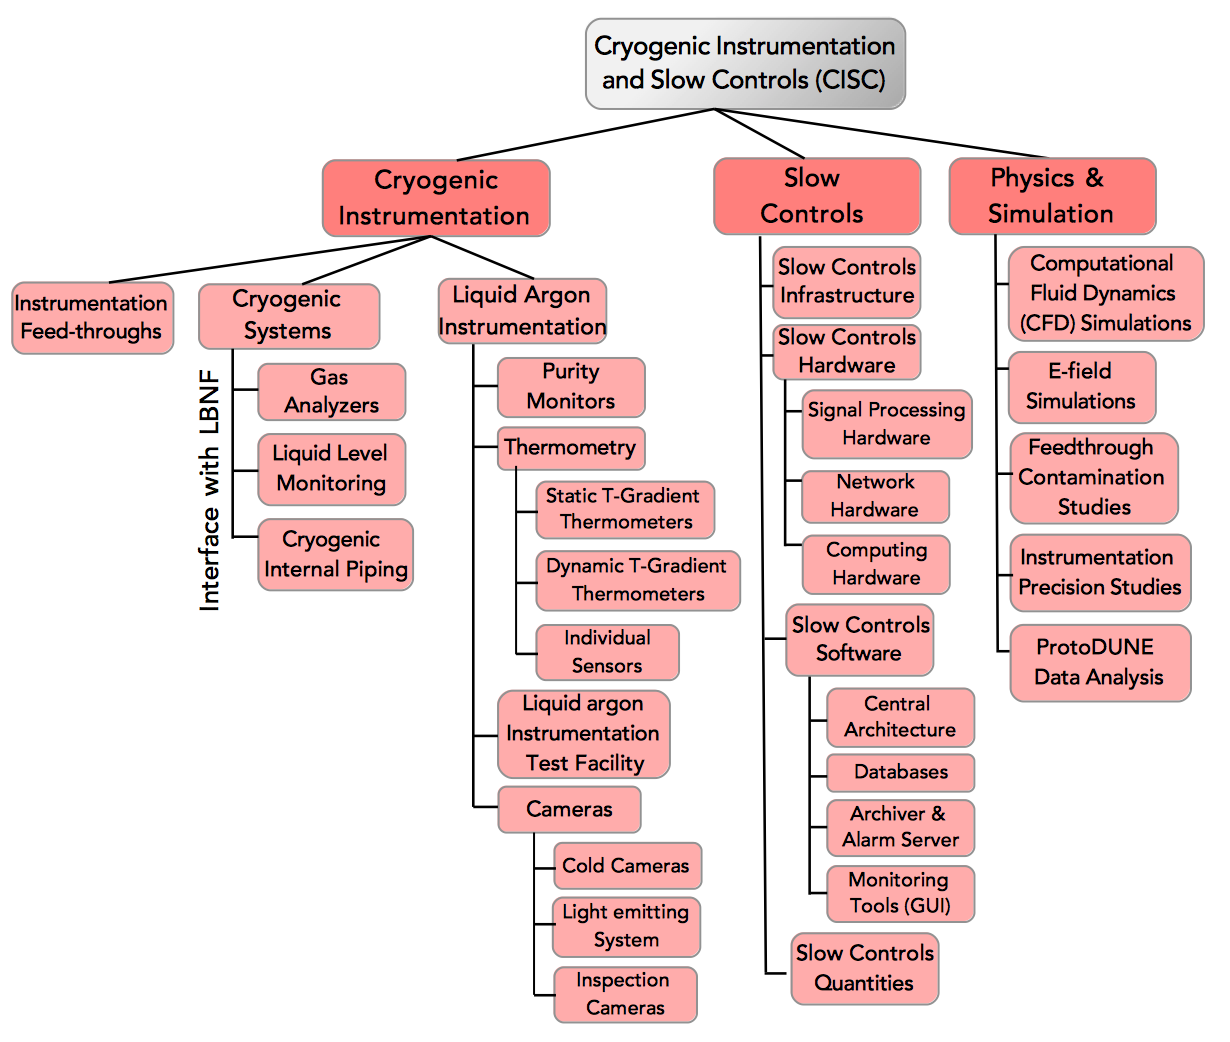
\includegraphics[width=0.7\textwidth]{fd-slow-cryo-subsys}
\end{dunefigure}

The instrumentation work related to gas analyzers, liquid level
monitors and cryostat internal cryogenic piping has significant
interface with LBNF and will be coordinated between DUNE and LBNF.
Cryogenic instrumentation also requires significant physics and
simulation work such as E-field simulations and cryogenics modeling
studies using Computational Fluid Dynamics (CFD). E-field simulations
are required to identify desirable locations for instrumentation
devices in the cryostat such that they are not near high E-fields and
that the designs do not induce large field distortions. CFD
simulations are needed to understand the expected temperature,
impurity and velocity flow distributions and guide the placement and
distribution of instrumentation devices inside the cryostat.


%%%%%%%%%%%%%%%%%%%%%%%%%%%%%%%%%%%%%
\subsection{Design Considerations}
\label{sec:fddp-slow-cryo-des-consid}

% specific to DP

For all liquid argon instrumentation devices, ProtoDUNE-DP designs are
considered as baseline designs and requirements for most design
parameters are extrapolated from ProtoDUNE. Hence a critical step for
the CISC consortium is to analyze data from ProtoDUNE when available
to validate the instrumentation designs and understand their
performance. Some of the common design considerations for
instrumentation devices include stability, reliability and longevity
such that the devices can survive for a period of at least 20 years
(current official DUNE run time).  Since it is uncommon for any device
to have such a long lifetime, provisions will be made in the overall
design to allow replacement of devices after certain number of
years. The noise from instrumentation devices need to be kept at the
ALARA level where ALARA stands for As Low As Reasonably
Achievable. The electric fields near the instrumentation devices are required
to be less than \SI{30}{kV\per\cm} or lower. Given the impossibility
of finding locations of low electric potential in a DP detector,
electric field shielding will be required for instrumentation
devices. Another common consideration for all instrumentation devices
is the support structure design which is expected to be substantially
different from ProtoDUNE.

For slow controls, the system needs to be designed such that it is
robust enough to support large number of variables, broad range of
monitoring and archiving rates and has the capability to interface
with large number of systems to establish two-way communication for
control and monitoring. Table \ref{tab:dp-cisc-requirements} shows
some of the important CISC system design requirements.

%A full list of
% requirements for design parameters can be found in DUNE Doc-DB 6440.



\begin{dunetable}
[Important design requirements on the DP CISC system design]
{p{0.3\textwidth}p{0.18\textwidth}p{0.42\textwidth}}
{tab:dp-cisc-requirements}
{Important design requirements on the dual phase CISC system design}   
Design Parameter
 & Requirement
 & Comment \\ \toprowrule
Electron lifetime measurement precision
 & $<\SI{1.4}{\%}$
 & Per DUNE-FD Task Force, needed to keep the bias on the charge readout in the TPC to below \SI{0.5}{\%} at \SI{3}{ms}\\  \colhline
Thermometers precision
 & $<\SI{5}{mK}$
 & Driven by CFD simulation validation; based on ProtoDUNE-SP design \\ \colhline
Liquid level meters precision
 & \SI{0.1}{\%} over \SI{14}{m}
 & Standard sensitivity; will use two level meters for redundancy \\  \colhline
Cryogenic Instrumentation Test Facility volume
 & 0.5 to \SI{3}{m^3}
 & Based on filling costs and turn around times \\  \colhline
Alarm rate
 & \(<\SI{150}{\per\day}\)
 & Recommended manageable alarm rate; allows experiment operators to respond to every alarm. \\  \colhline
Total no.\ of variables
 & 50k to 100k
 & Expected number based on scaling past experiments; requires robust base software model that can handle large no. of variables. \\  \colhline
Archiving rate
 & 1 Hz to \(\SI{0.3}{\per\minute}\)
 & Based on expected rapidity of interesting changes; impacts the base software model choice; will depend on data storage capabilities \\ \colhline
Near Detector  status
 & Full Beam and Detector Status
 & Operate DUNE as one experiment. \\
% 
% 
% 
% Requirement  
%   \\ \colhline
%    \\ \colhline
%  ...\\ 
\end{dunetable}

\fixme{By the end of the volume, for every requirement listed in this section, there should exist an explanation of how it will be satisfied.}


%%%%%%%%%%%%%%%%%%%%%%%%%%%%%%%%
\subsection{Scope}
\label{sec:fddp-slow-cryo-scope}

% identical for SP and DP

The scope of the CISC system spans broad range of activities. In the
case of Cryogenics Systems (gas analyzers, liquid level monitors and
cryogenic internal piping), LBNF will provide the needed expertise and
is responsible for the design, installation and commissioning activities
while the CISC consortium provides the cost and supplement the labor as
needed. In the case of instrumentation devices (purity monitors,
thermometers, cameras, and light emitting system) and instrumentation
test facility, CISC will be responsible from design to commissioning in
the far detectors.

From the slow controls side, CISC will provide control and monitoring of
all detector elements that provide information on the health of the
detector or conditions important to the experiment. The scope of slow
controls quantities includes,

\begin{itemize}
\item
  Full rack monitoring (rack fans, thermometers and rack protection
  system); 
\item
  Interlock status bit monitoring (not the actual interlock mechanism)
\item
  Building controls; Detector hall monitoring; ground impedance
  monitoring
\item
  Monitoring and control for all power supplies
\item
  Detector components inspection through warm cameras
\item
  High voltage system monitoring through cold cameras
\item
  Beam status; Cryogenics status; DAQ status; 
\item
  Power distribution units monitoring; Computer hardware monitoring
\item
  Instrumentation and Calibration device monitoring (and control to the
  extent needed)
\item
  Alarms; archiving; display panels; operator interface tools 
\item
  Slow controls system documentation and operations guidelines
\end{itemize}

In terms of slow controls hardware, CISC will develop, install and
commission any hardware related to rack monitoring and control. While
most power supplies might only need a cable from the device to an
ethernet switch, some power supplies might need special cables (e.g.
GPIB or RS232) for communication. The CISC consortium is responsible for
buying such control cables.

In addition to the listed activities, CISC also has activities that span
outside the scope of the consortium and require interfacing with other
groups.

% More specific information on how CISC scope of activities
% interface with other consortia can be found at DUNE Doc-dbs 6679 (APA),
% 6730 (SP-PD), 6745 (SP-CE), 6760 (DP-CRP), 6781 (DP-PD), 6784 (DP-CE),
% 6787 (HV), and 6790 (DAQ). The CISC interface documents with facility,
% installation, integration, calibration, and physics can be found at DUNE
% Doc-dbs 6991, 7018, 7045, 7072, and 7099, respectively. The CISC
% interface document with software and computing can be found at DUNE
% Doc-db 7126.
